\documentclass[twoside]{book}

% Packages required by doxygen
\usepackage{fixltx2e}
\usepackage{calc}
\usepackage{doxygen}
\usepackage[export]{adjustbox} % also loads graphicx
\usepackage{graphicx}
\usepackage[utf8]{inputenc}
\usepackage{makeidx}
\usepackage{multicol}
\usepackage{multirow}
\PassOptionsToPackage{warn}{textcomp}
\usepackage{textcomp}
\usepackage[nointegrals]{wasysym}
\usepackage[table]{xcolor}

% Font selection
\usepackage[T1]{fontenc}
\usepackage[scaled=.90]{helvet}
\usepackage{courier}
\usepackage{amssymb}
\usepackage{sectsty}
\renewcommand{\familydefault}{\sfdefault}
\allsectionsfont{%
  \fontseries{bc}\selectfont%
  \color{darkgray}%
}
\renewcommand{\DoxyLabelFont}{%
  \fontseries{bc}\selectfont%
  \color{darkgray}%
}
\newcommand{\+}{\discretionary{\mbox{\scriptsize$\hookleftarrow$}}{}{}}

% Page & text layout
\usepackage{geometry}
\geometry{%
  a4paper,%
  top=2.5cm,%
  bottom=2.5cm,%
  left=2.5cm,%
  right=2.5cm%
}
\tolerance=750
\hfuzz=15pt
\hbadness=750
\setlength{\emergencystretch}{15pt}
\setlength{\parindent}{0cm}
\setlength{\parskip}{3ex plus 2ex minus 2ex}
\makeatletter
\renewcommand{\paragraph}{%
  \@startsection{paragraph}{4}{0ex}{-1.0ex}{1.0ex}{%
    \normalfont\normalsize\bfseries\SS@parafont%
  }%
}
\renewcommand{\subparagraph}{%
  \@startsection{subparagraph}{5}{0ex}{-1.0ex}{1.0ex}{%
    \normalfont\normalsize\bfseries\SS@subparafont%
  }%
}
\makeatother

% Headers & footers
\usepackage{fancyhdr}
\pagestyle{fancyplain}
\fancyhead[LE]{\fancyplain{}{\bfseries\thepage}}
\fancyhead[CE]{\fancyplain{}{}}
\fancyhead[RE]{\fancyplain{}{\bfseries\leftmark}}
\fancyhead[LO]{\fancyplain{}{\bfseries\rightmark}}
\fancyhead[CO]{\fancyplain{}{}}
\fancyhead[RO]{\fancyplain{}{\bfseries\thepage}}
\fancyfoot[LE]{\fancyplain{}{}}
\fancyfoot[CE]{\fancyplain{}{}}
\fancyfoot[RE]{\fancyplain{}{\bfseries\scriptsize Generated by Doxygen }}
\fancyfoot[LO]{\fancyplain{}{\bfseries\scriptsize Generated by Doxygen }}
\fancyfoot[CO]{\fancyplain{}{}}
\fancyfoot[RO]{\fancyplain{}{}}
\renewcommand{\footrulewidth}{0.4pt}
\renewcommand{\chaptermark}[1]{%
  \markboth{#1}{}%
}
\renewcommand{\sectionmark}[1]{%
  \markright{\thesection\ #1}%
}

% Indices & bibliography
\usepackage{natbib}
\usepackage[titles]{tocloft}
\setcounter{tocdepth}{3}
\setcounter{secnumdepth}{5}
\makeindex

% Hyperlinks (required, but should be loaded last)
\usepackage{ifpdf}
\ifpdf
  \usepackage[pdftex,pagebackref=true]{hyperref}
\else
  \usepackage[ps2pdf,pagebackref=true]{hyperref}
\fi
\hypersetup{%
  colorlinks=true,%
  linkcolor=blue,%
  citecolor=blue,%
  unicode%
}

% Custom commands
\newcommand{\clearemptydoublepage}{%
  \newpage{\pagestyle{empty}\cleardoublepage}%
}

\usepackage{caption}
\captionsetup{labelsep=space,justification=centering,font={bf},singlelinecheck=off,skip=4pt,position=top}

%===== C O N T E N T S =====

\begin{document}

% Titlepage & ToC
\hypersetup{pageanchor=false,
             bookmarksnumbered=true,
             pdfencoding=unicode
            }
\pagenumbering{roman}
\begin{titlepage}
\vspace*{7cm}
\begin{center}%
{\Large Architect Class }\\
\vspace*{1cm}
{\large Generated by Doxygen 1.8.11}\\
\end{center}
\end{titlepage}
\clearemptydoublepage
\tableofcontents
\clearemptydoublepage
\pagenumbering{arabic}
\hypersetup{pageanchor=true}

%--- Begin generated contents ---
\chapter{Hierarchical Index}
\section{Class Hierarchy}
This inheritance list is sorted roughly, but not completely, alphabetically\+:\begin{DoxyCompactList}
\item \contentsline{section}{My\+App\textbackslash{}Controller}{\pageref{class_my_app_1_1_controller}}{}
\begin{DoxyCompactList}
\item \contentsline{section}{My\+App\textbackslash{}Controller\textbackslash{}Index}{\pageref{class_my_app_1_1_controller_1_1_index}}{}
\item \contentsline{section}{My\+App\textbackslash{}Controller\textbackslash{}Login}{\pageref{class_my_app_1_1_controller_1_1_login}}{}
\item \contentsline{section}{My\+App\textbackslash{}Controller\textbackslash{}Signup}{\pageref{class_my_app_1_1_controller_1_1_signup}}{}
\end{DoxyCompactList}
\item Exception\begin{DoxyCompactList}
\item \contentsline{section}{My\+App\textbackslash{}Exception\textbackslash{}Duplicate\+Email}{\pageref{class_my_app_1_1_exception_1_1_duplicate_email}}{}
\item \contentsline{section}{My\+App\textbackslash{}Exception\textbackslash{}Empty\+Post}{\pageref{class_my_app_1_1_exception_1_1_empty_post}}{}
\item \contentsline{section}{My\+App\textbackslash{}Exception\textbackslash{}Invalid\+Email}{\pageref{class_my_app_1_1_exception_1_1_invalid_email}}{}
\item \contentsline{section}{My\+App\textbackslash{}Exception\textbackslash{}Invalid\+Password}{\pageref{class_my_app_1_1_exception_1_1_invalid_password}}{}
\item \contentsline{section}{My\+App\textbackslash{}Exception\textbackslash{}Unmatch\+Email\+Or\+Password}{\pageref{class_my_app_1_1_exception_1_1_unmatch_email_or_password}}{}
\end{DoxyCompactList}
\item \contentsline{section}{My\+App\textbackslash{}Model}{\pageref{class_my_app_1_1_model}}{}
\begin{DoxyCompactList}
\item \contentsline{section}{My\+App\textbackslash{}Model\textbackslash{}User}{\pageref{class_my_app_1_1_model_1_1_user}}{}
\end{DoxyCompactList}
\end{DoxyCompactList}

\chapter{Class Index}
\section{Class List}
Here are the classes, structs, unions and interfaces with brief descriptions\+:\begin{DoxyCompactList}
\item\contentsline{section}{\hyperlink{class_my_app_1_1_controller}{My\+App\textbackslash{}\+Controller} }{\pageref{class_my_app_1_1_controller}}{}
\item\contentsline{section}{\hyperlink{class_my_app_1_1_exception_1_1_duplicate_email}{My\+App\textbackslash{}\+Exception\textbackslash{}\+Duplicate\+Email} }{\pageref{class_my_app_1_1_exception_1_1_duplicate_email}}{}
\item\contentsline{section}{\hyperlink{class_my_app_1_1_exception_1_1_empty_post}{My\+App\textbackslash{}\+Exception\textbackslash{}\+Empty\+Post} }{\pageref{class_my_app_1_1_exception_1_1_empty_post}}{}
\item\contentsline{section}{\hyperlink{class_my_app_1_1_controller_1_1_index}{My\+App\textbackslash{}\+Controller\textbackslash{}\+Index} }{\pageref{class_my_app_1_1_controller_1_1_index}}{}
\item\contentsline{section}{\hyperlink{class_my_app_1_1_exception_1_1_invalid_email}{My\+App\textbackslash{}\+Exception\textbackslash{}\+Invalid\+Email} }{\pageref{class_my_app_1_1_exception_1_1_invalid_email}}{}
\item\contentsline{section}{\hyperlink{class_my_app_1_1_exception_1_1_invalid_password}{My\+App\textbackslash{}\+Exception\textbackslash{}\+Invalid\+Password} }{\pageref{class_my_app_1_1_exception_1_1_invalid_password}}{}
\item\contentsline{section}{\hyperlink{class_my_app_1_1_controller_1_1_login}{My\+App\textbackslash{}\+Controller\textbackslash{}\+Login} }{\pageref{class_my_app_1_1_controller_1_1_login}}{}
\item\contentsline{section}{\hyperlink{class_my_app_1_1_model}{My\+App\textbackslash{}\+Model} }{\pageref{class_my_app_1_1_model}}{}
\item\contentsline{section}{\hyperlink{class_my_app_1_1_controller_1_1_signup}{My\+App\textbackslash{}\+Controller\textbackslash{}\+Signup} }{\pageref{class_my_app_1_1_controller_1_1_signup}}{}
\item\contentsline{section}{\hyperlink{class_my_app_1_1_exception_1_1_unmatch_email_or_password}{My\+App\textbackslash{}\+Exception\textbackslash{}\+Unmatch\+Email\+Or\+Password} }{\pageref{class_my_app_1_1_exception_1_1_unmatch_email_or_password}}{}
\item\contentsline{section}{\hyperlink{class_my_app_1_1_model_1_1_user}{My\+App\textbackslash{}\+Model\textbackslash{}\+User} }{\pageref{class_my_app_1_1_model_1_1_user}}{}
\end{DoxyCompactList}

\chapter{Class Documentation}
\hypertarget{class_my_app_1_1_controller}{}\section{My\+App\textbackslash{}Controller Class Reference}
\label{class_my_app_1_1_controller}\index{My\+App\textbackslash{}\+Controller@{My\+App\textbackslash{}\+Controller}}


Inheritance diagram for My\+App\textbackslash{}Controller\+:
\nopagebreak
\begin{figure}[H]
\begin{center}
\leavevmode
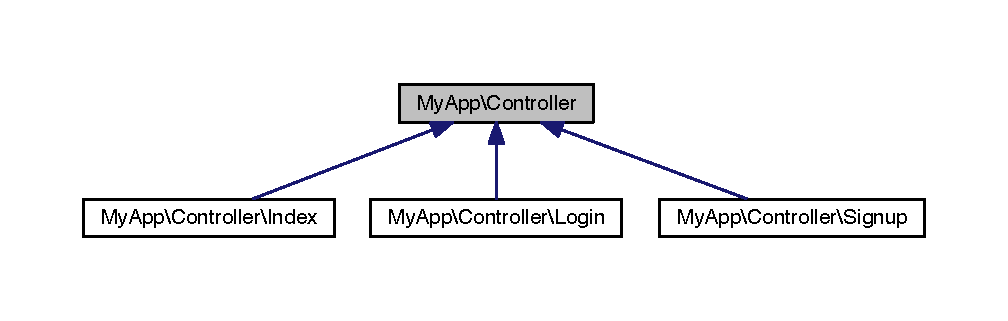
\includegraphics[width=350pt]{class_my_app_1_1_controller__inherit__graph}
\end{center}
\end{figure}
\subsection*{Public Member Functions}
\begin{DoxyCompactItemize}
\item 
{\bfseries get\+Values} ()\hypertarget{class_my_app_1_1_controller_aed15f2fb497e55d07f80c7a709c89943}{}\label{class_my_app_1_1_controller_aed15f2fb497e55d07f80c7a709c89943}

\item 
{\bfseries get\+Errors} (\$key)\hypertarget{class_my_app_1_1_controller_a43bd03dfa3857358733da41dabc3beea}{}\label{class_my_app_1_1_controller_a43bd03dfa3857358733da41dabc3beea}

\item 
{\bfseries me} ()\hypertarget{class_my_app_1_1_controller_aa8bbf0425e272480670e0e01a32ef6bb}{}\label{class_my_app_1_1_controller_aa8bbf0425e272480670e0e01a32ef6bb}

\end{DoxyCompactItemize}
\subsection*{Protected Member Functions}
\begin{DoxyCompactItemize}
\item 
{\bfseries set\+Values} (\$key, \$value)\hypertarget{class_my_app_1_1_controller_a3b888e7de66b3312578c959b3af94335}{}\label{class_my_app_1_1_controller_a3b888e7de66b3312578c959b3af94335}

\item 
{\bfseries set\+Errors} (\$key, \$error)\hypertarget{class_my_app_1_1_controller_ad26ce27e010db6e3658d3b943b61c589}{}\label{class_my_app_1_1_controller_ad26ce27e010db6e3658d3b943b61c589}

\item 
{\bfseries has\+Error} ()\hypertarget{class_my_app_1_1_controller_a0eb5c57d99ad6b38090a8f3ff2a8071a}{}\label{class_my_app_1_1_controller_a0eb5c57d99ad6b38090a8f3ff2a8071a}

\item 
{\bfseries is\+Logged\+In} ()\hypertarget{class_my_app_1_1_controller_aec09ecacd0354a680655a470f17a4135}{}\label{class_my_app_1_1_controller_aec09ecacd0354a680655a470f17a4135}

\end{DoxyCompactItemize}


The documentation for this class was generated from the following file\+:\begin{DoxyCompactItemize}
\item 
lib/Controller.\+php\end{DoxyCompactItemize}

\hypertarget{class_my_app_1_1_exception_1_1_duplicate_email}{}\section{My\+App\textbackslash{}Exception\textbackslash{}Duplicate\+Email Class Reference}
\label{class_my_app_1_1_exception_1_1_duplicate_email}\index{My\+App\textbackslash{}\+Exception\textbackslash{}\+Duplicate\+Email@{My\+App\textbackslash{}\+Exception\textbackslash{}\+Duplicate\+Email}}


Inheritance diagram for My\+App\textbackslash{}Exception\textbackslash{}Duplicate\+Email\+:
\nopagebreak
\begin{figure}[H]
\begin{center}
\leavevmode
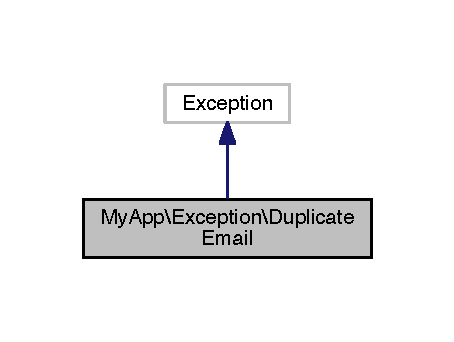
\includegraphics[width=218pt]{class_my_app_1_1_exception_1_1_duplicate_email__inherit__graph}
\end{center}
\end{figure}


Collaboration diagram for My\+App\textbackslash{}Exception\textbackslash{}Duplicate\+Email\+:
\nopagebreak
\begin{figure}[H]
\begin{center}
\leavevmode
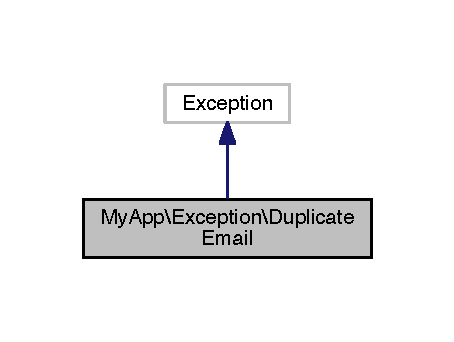
\includegraphics[width=218pt]{class_my_app_1_1_exception_1_1_duplicate_email__coll__graph}
\end{center}
\end{figure}
\subsection*{Protected Attributes}
\begin{DoxyCompactItemize}
\item 
{\bfseries \$message} = \textquotesingle{}Duplicate Email!\textquotesingle{}\hypertarget{class_my_app_1_1_exception_1_1_duplicate_email_aefe80876a9c577da6cc4653308b244a5}{}\label{class_my_app_1_1_exception_1_1_duplicate_email_aefe80876a9c577da6cc4653308b244a5}

\end{DoxyCompactItemize}


The documentation for this class was generated from the following file\+:\begin{DoxyCompactItemize}
\item 
lib/\+Exception/Duplicate\+Email.\+php\end{DoxyCompactItemize}

\hypertarget{class_my_app_1_1_exception_1_1_empty_post}{}\section{My\+App\textbackslash{}Exception\textbackslash{}Empty\+Post Class Reference}
\label{class_my_app_1_1_exception_1_1_empty_post}\index{My\+App\textbackslash{}\+Exception\textbackslash{}\+Empty\+Post@{My\+App\textbackslash{}\+Exception\textbackslash{}\+Empty\+Post}}


Inheritance diagram for My\+App\textbackslash{}Exception\textbackslash{}Empty\+Post\+:
\nopagebreak
\begin{figure}[H]
\begin{center}
\leavevmode
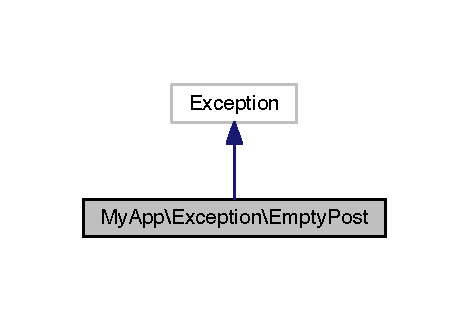
\includegraphics[width=225pt]{class_my_app_1_1_exception_1_1_empty_post__inherit__graph}
\end{center}
\end{figure}


Collaboration diagram for My\+App\textbackslash{}Exception\textbackslash{}Empty\+Post\+:
\nopagebreak
\begin{figure}[H]
\begin{center}
\leavevmode
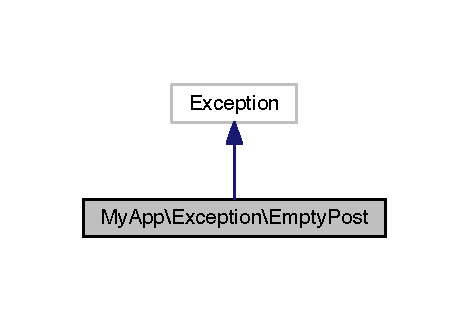
\includegraphics[width=225pt]{class_my_app_1_1_exception_1_1_empty_post__coll__graph}
\end{center}
\end{figure}
\subsection*{Protected Attributes}
\begin{DoxyCompactItemize}
\item 
{\bfseries \$message} = \textquotesingle{}Please enter email/password!\textquotesingle{}\hypertarget{class_my_app_1_1_exception_1_1_empty_post_a038f2653142cf871d1b0226b8d404d7d}{}\label{class_my_app_1_1_exception_1_1_empty_post_a038f2653142cf871d1b0226b8d404d7d}

\end{DoxyCompactItemize}


The documentation for this class was generated from the following file\+:\begin{DoxyCompactItemize}
\item 
lib/\+Exception/Empty\+Post.\+php\end{DoxyCompactItemize}

\hypertarget{class_my_app_1_1_controller_1_1_index}{}\section{My\+App\textbackslash{}Controller\textbackslash{}Index Class Reference}
\label{class_my_app_1_1_controller_1_1_index}\index{My\+App\textbackslash{}\+Controller\textbackslash{}\+Index@{My\+App\textbackslash{}\+Controller\textbackslash{}\+Index}}


Inheritance diagram for My\+App\textbackslash{}Controller\textbackslash{}Index\+:\nopagebreak
\begin{figure}[H]
\begin{center}
\leavevmode
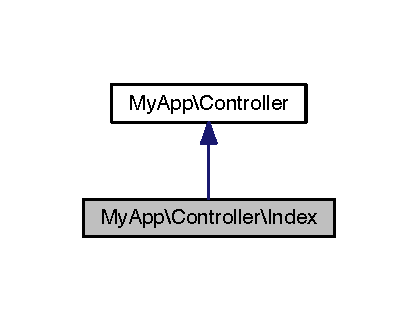
\includegraphics[width=200pt]{class_my_app_1_1_controller_1_1_index__inherit__graph}
\end{center}
\end{figure}


Collaboration diagram for My\+App\textbackslash{}Controller\textbackslash{}Index\+:\nopagebreak
\begin{figure}[H]
\begin{center}
\leavevmode
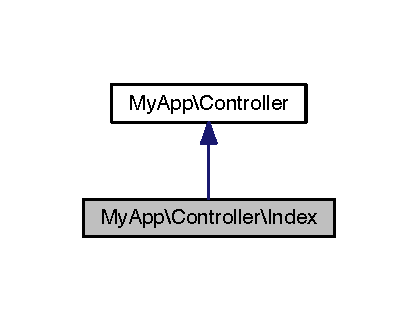
\includegraphics[width=200pt]{class_my_app_1_1_controller_1_1_index__coll__graph}
\end{center}
\end{figure}
\subsection*{Public Member Functions}
\begin{DoxyCompactItemize}
\item 
{\bfseries run} ()\hypertarget{class_my_app_1_1_controller_1_1_index_aca982083dce827dd3d58199f587ef792}{}\label{class_my_app_1_1_controller_1_1_index_aca982083dce827dd3d58199f587ef792}

\end{DoxyCompactItemize}
\subsection*{Additional Inherited Members}


The documentation for this class was generated from the following file\+:\begin{DoxyCompactItemize}
\item 
lib/controller/Index.\+php\end{DoxyCompactItemize}

\hypertarget{class_my_app_1_1_exception_1_1_invalid_email}{}\section{My\+App\textbackslash{}Exception\textbackslash{}Invalid\+Email Class Reference}
\label{class_my_app_1_1_exception_1_1_invalid_email}\index{My\+App\textbackslash{}\+Exception\textbackslash{}\+Invalid\+Email@{My\+App\textbackslash{}\+Exception\textbackslash{}\+Invalid\+Email}}


Inheritance diagram for My\+App\textbackslash{}Exception\textbackslash{}Invalid\+Email\+:
\nopagebreak
\begin{figure}[H]
\begin{center}
\leavevmode
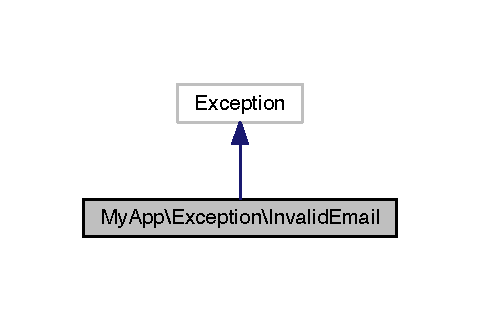
\includegraphics[width=231pt]{class_my_app_1_1_exception_1_1_invalid_email__inherit__graph}
\end{center}
\end{figure}


Collaboration diagram for My\+App\textbackslash{}Exception\textbackslash{}Invalid\+Email\+:
\nopagebreak
\begin{figure}[H]
\begin{center}
\leavevmode
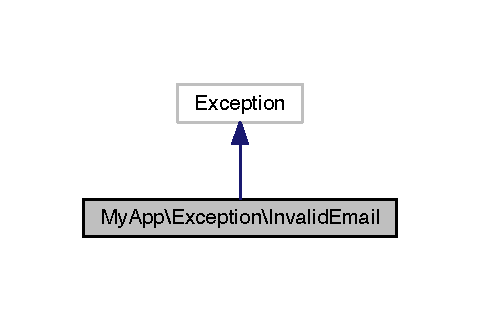
\includegraphics[width=231pt]{class_my_app_1_1_exception_1_1_invalid_email__coll__graph}
\end{center}
\end{figure}
\subsection*{Protected Attributes}
\begin{DoxyCompactItemize}
\item 
{\bfseries \$message} = \textquotesingle{}Invalid Email!\textquotesingle{}\hypertarget{class_my_app_1_1_exception_1_1_invalid_email_a555474638aaec584514e6a8f305787ab}{}\label{class_my_app_1_1_exception_1_1_invalid_email_a555474638aaec584514e6a8f305787ab}

\end{DoxyCompactItemize}


The documentation for this class was generated from the following file\+:\begin{DoxyCompactItemize}
\item 
lib/\+Exception/Invalid\+Email.\+php\end{DoxyCompactItemize}

\hypertarget{class_my_app_1_1_exception_1_1_invalid_password}{}\section{My\+App\textbackslash{}Exception\textbackslash{}Invalid\+Password Class Reference}
\label{class_my_app_1_1_exception_1_1_invalid_password}\index{My\+App\textbackslash{}\+Exception\textbackslash{}\+Invalid\+Password@{My\+App\textbackslash{}\+Exception\textbackslash{}\+Invalid\+Password}}


Inheritance diagram for My\+App\textbackslash{}Exception\textbackslash{}Invalid\+Password\+:
\nopagebreak
\begin{figure}[H]
\begin{center}
\leavevmode
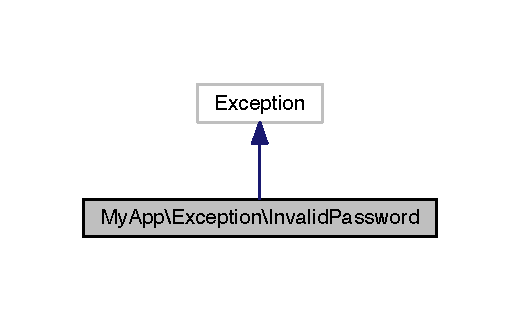
\includegraphics[width=249pt]{class_my_app_1_1_exception_1_1_invalid_password__inherit__graph}
\end{center}
\end{figure}


Collaboration diagram for My\+App\textbackslash{}Exception\textbackslash{}Invalid\+Password\+:
\nopagebreak
\begin{figure}[H]
\begin{center}
\leavevmode
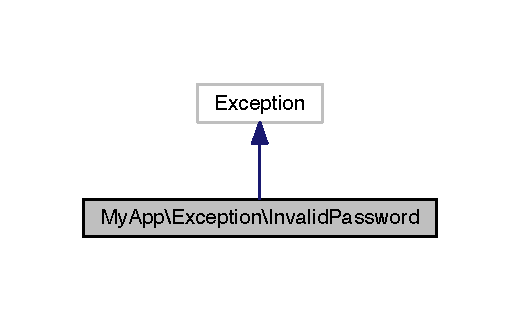
\includegraphics[width=249pt]{class_my_app_1_1_exception_1_1_invalid_password__coll__graph}
\end{center}
\end{figure}
\subsection*{Protected Attributes}
\begin{DoxyCompactItemize}
\item 
{\bfseries \$message} = \textquotesingle{}Invalid Password!\textquotesingle{}\hypertarget{class_my_app_1_1_exception_1_1_invalid_password_a22827c681fe61dd1d527bba299dba443}{}\label{class_my_app_1_1_exception_1_1_invalid_password_a22827c681fe61dd1d527bba299dba443}

\end{DoxyCompactItemize}


The documentation for this class was generated from the following file\+:\begin{DoxyCompactItemize}
\item 
lib/\+Exception/Invalid\+Password.\+php\end{DoxyCompactItemize}

\hypertarget{class_my_app_1_1_controller_1_1_login}{}\section{My\+App\textbackslash{}Controller\textbackslash{}Login Class Reference}
\label{class_my_app_1_1_controller_1_1_login}\index{My\+App\textbackslash{}\+Controller\textbackslash{}\+Login@{My\+App\textbackslash{}\+Controller\textbackslash{}\+Login}}


Inheritance diagram for My\+App\textbackslash{}Controller\textbackslash{}Login\+:
\nopagebreak
\begin{figure}[H]
\begin{center}
\leavevmode
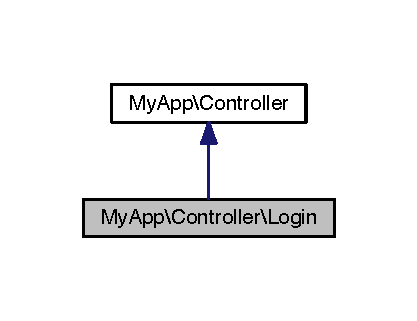
\includegraphics[width=200pt]{class_my_app_1_1_controller_1_1_login__inherit__graph}
\end{center}
\end{figure}


Collaboration diagram for My\+App\textbackslash{}Controller\textbackslash{}Login\+:
\nopagebreak
\begin{figure}[H]
\begin{center}
\leavevmode
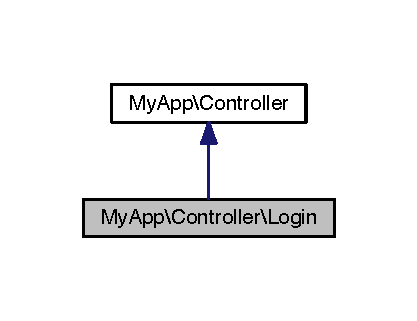
\includegraphics[width=200pt]{class_my_app_1_1_controller_1_1_login__coll__graph}
\end{center}
\end{figure}
\subsection*{Public Member Functions}
\begin{DoxyCompactItemize}
\item 
{\bfseries run} ()\hypertarget{class_my_app_1_1_controller_1_1_login_aa0bc28e2af0d0d3aaa9231e18744b8ce}{}\label{class_my_app_1_1_controller_1_1_login_aa0bc28e2af0d0d3aaa9231e18744b8ce}

\end{DoxyCompactItemize}
\subsection*{Protected Member Functions}
\begin{DoxyCompactItemize}
\item 
{\bfseries post\+Process} ()\hypertarget{class_my_app_1_1_controller_1_1_login_a2ce27ddc079690184240b34c12d541fb}{}\label{class_my_app_1_1_controller_1_1_login_a2ce27ddc079690184240b34c12d541fb}

\end{DoxyCompactItemize}


The documentation for this class was generated from the following file\+:\begin{DoxyCompactItemize}
\item 
lib/controller/Login.\+php\end{DoxyCompactItemize}

\hypertarget{class_my_app_1_1_model}{}\section{My\+App\textbackslash{}Model Class Reference}
\label{class_my_app_1_1_model}\index{My\+App\textbackslash{}\+Model@{My\+App\textbackslash{}\+Model}}


Inheritance diagram for My\+App\textbackslash{}Model\+:\nopagebreak
\begin{figure}[H]
\begin{center}
\leavevmode
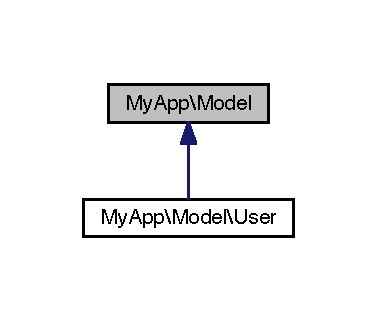
\includegraphics[width=181pt]{class_my_app_1_1_model__inherit__graph}
\end{center}
\end{figure}
\subsection*{Protected Attributes}
\begin{DoxyCompactItemize}
\item 
{\bfseries \$db}\hypertarget{class_my_app_1_1_model_a59413d5b8ddb51939c3d841bfd5d7695}{}\label{class_my_app_1_1_model_a59413d5b8ddb51939c3d841bfd5d7695}

\end{DoxyCompactItemize}


The documentation for this class was generated from the following file\+:\begin{DoxyCompactItemize}
\item 
lib/Model.\+php\end{DoxyCompactItemize}

\hypertarget{class_my_app_1_1_controller_1_1_signup}{}\section{My\+App\textbackslash{}Controller\textbackslash{}Signup Class Reference}
\label{class_my_app_1_1_controller_1_1_signup}\index{My\+App\textbackslash{}\+Controller\textbackslash{}\+Signup@{My\+App\textbackslash{}\+Controller\textbackslash{}\+Signup}}


Inheritance diagram for My\+App\textbackslash{}Controller\textbackslash{}Signup\+:
\nopagebreak
\begin{figure}[H]
\begin{center}
\leavevmode
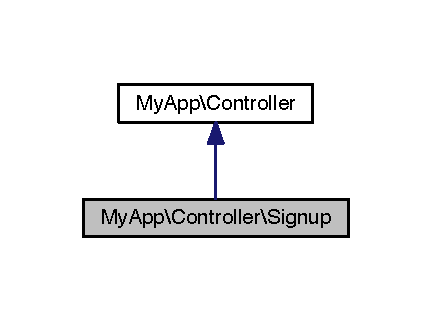
\includegraphics[width=207pt]{class_my_app_1_1_controller_1_1_signup__inherit__graph}
\end{center}
\end{figure}


Collaboration diagram for My\+App\textbackslash{}Controller\textbackslash{}Signup\+:
\nopagebreak
\begin{figure}[H]
\begin{center}
\leavevmode
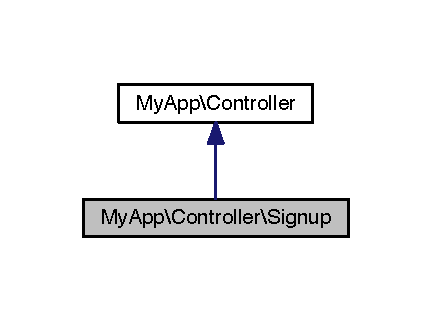
\includegraphics[width=207pt]{class_my_app_1_1_controller_1_1_signup__coll__graph}
\end{center}
\end{figure}
\subsection*{Public Member Functions}
\begin{DoxyCompactItemize}
\item 
{\bfseries run} ()\hypertarget{class_my_app_1_1_controller_1_1_signup_a6b4394b3505a26084fdebe7cc5757c3c}{}\label{class_my_app_1_1_controller_1_1_signup_a6b4394b3505a26084fdebe7cc5757c3c}

\end{DoxyCompactItemize}
\subsection*{Protected Member Functions}
\begin{DoxyCompactItemize}
\item 
{\bfseries post\+Process} ()\hypertarget{class_my_app_1_1_controller_1_1_signup_a98b7f8744c8d0a160b655b91208942d5}{}\label{class_my_app_1_1_controller_1_1_signup_a98b7f8744c8d0a160b655b91208942d5}

\end{DoxyCompactItemize}


The documentation for this class was generated from the following file\+:\begin{DoxyCompactItemize}
\item 
lib/controller/Signup.\+php\end{DoxyCompactItemize}

\hypertarget{class_my_app_1_1_exception_1_1_unmatch_email_or_password}{}\section{My\+App\textbackslash{}Exception\textbackslash{}Unmatch\+Email\+Or\+Password Class Reference}
\label{class_my_app_1_1_exception_1_1_unmatch_email_or_password}\index{My\+App\textbackslash{}\+Exception\textbackslash{}\+Unmatch\+Email\+Or\+Password@{My\+App\textbackslash{}\+Exception\textbackslash{}\+Unmatch\+Email\+Or\+Password}}


Inheritance diagram for My\+App\textbackslash{}Exception\textbackslash{}Unmatch\+Email\+Or\+Password\+:
\nopagebreak
\begin{figure}[H]
\begin{center}
\leavevmode
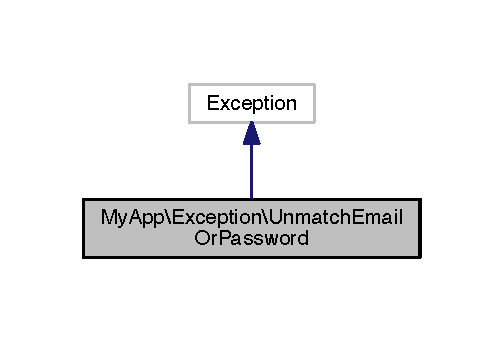
\includegraphics[width=242pt]{class_my_app_1_1_exception_1_1_unmatch_email_or_password__inherit__graph}
\end{center}
\end{figure}


Collaboration diagram for My\+App\textbackslash{}Exception\textbackslash{}Unmatch\+Email\+Or\+Password\+:
\nopagebreak
\begin{figure}[H]
\begin{center}
\leavevmode
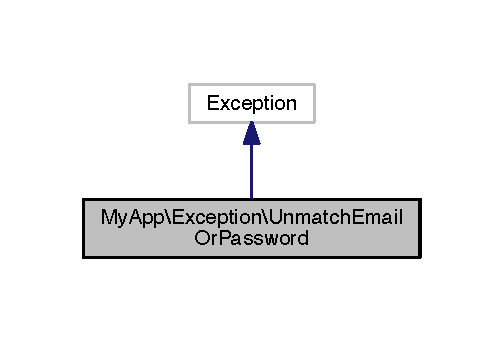
\includegraphics[width=242pt]{class_my_app_1_1_exception_1_1_unmatch_email_or_password__coll__graph}
\end{center}
\end{figure}
\subsection*{Protected Attributes}
\begin{DoxyCompactItemize}
\item 
{\bfseries \$message} = \textquotesingle{}Email/Password do not match!\textquotesingle{}\hypertarget{class_my_app_1_1_exception_1_1_unmatch_email_or_password_a034c1f2523c80dd4050626189d5c3340}{}\label{class_my_app_1_1_exception_1_1_unmatch_email_or_password_a034c1f2523c80dd4050626189d5c3340}

\end{DoxyCompactItemize}


The documentation for this class was generated from the following file\+:\begin{DoxyCompactItemize}
\item 
lib/\+Exception/Unmatch\+Email\+Or\+Password.\+php\end{DoxyCompactItemize}

\hypertarget{class_my_app_1_1_model_1_1_user}{}\section{My\+App\textbackslash{}Model\textbackslash{}User Class Reference}
\label{class_my_app_1_1_model_1_1_user}\index{My\+App\textbackslash{}\+Model\textbackslash{}\+User@{My\+App\textbackslash{}\+Model\textbackslash{}\+User}}


Inheritance diagram for My\+App\textbackslash{}Model\textbackslash{}User\+:\nopagebreak
\begin{figure}[H]
\begin{center}
\leavevmode
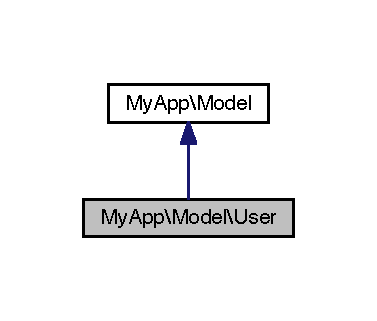
\includegraphics[width=181pt]{class_my_app_1_1_model_1_1_user__inherit__graph}
\end{center}
\end{figure}


Collaboration diagram for My\+App\textbackslash{}Model\textbackslash{}User\+:\nopagebreak
\begin{figure}[H]
\begin{center}
\leavevmode
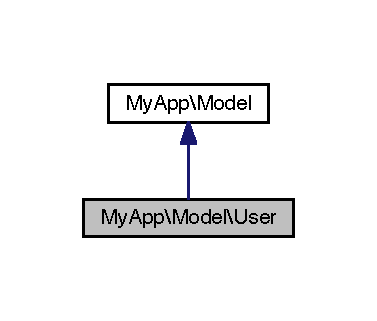
\includegraphics[width=181pt]{class_my_app_1_1_model_1_1_user__coll__graph}
\end{center}
\end{figure}
\subsection*{Public Member Functions}
\begin{DoxyCompactItemize}
\item 
{\bfseries create} (\$values)\hypertarget{class_my_app_1_1_model_1_1_user_acf5c0d1e8a2171c648f6ca5914b0dfce}{}\label{class_my_app_1_1_model_1_1_user_acf5c0d1e8a2171c648f6ca5914b0dfce}

\item 
{\bfseries login} (\$values)\hypertarget{class_my_app_1_1_model_1_1_user_a5b54bb950ece023acfc08574cb3c3500}{}\label{class_my_app_1_1_model_1_1_user_a5b54bb950ece023acfc08574cb3c3500}

\item 
{\bfseries find\+All} ()\hypertarget{class_my_app_1_1_model_1_1_user_a2c34790e418f92691854806e8ef6f819}{}\label{class_my_app_1_1_model_1_1_user_a2c34790e418f92691854806e8ef6f819}

\end{DoxyCompactItemize}
\subsection*{Additional Inherited Members}


The documentation for this class was generated from the following file\+:\begin{DoxyCompactItemize}
\item 
lib/\+Model/User.\+php\end{DoxyCompactItemize}

%--- End generated contents ---

% Index
\backmatter
\newpage
\phantomsection
\clearemptydoublepage
\addcontentsline{toc}{chapter}{Index}
\printindex

\end{document}
